\documentclass[../../main.tex]{subfiles}
\begin{document}

\section{Finite Elementer}

I finite element-metoden bygger vi opp funksjonsrom ved å sette sammen små byggeklosser kalt \emph{finitte elementer}. Hvert element beskriver funksjoner lokalt over et lite delområde av vårt totale domene. Dette reiser to fundamentale spørsmål:
\begin{itemize}
    \item Hvordan ser en funksjon ut over et enkelt element?
    \item Hvordan knyttes funksjoner sammen mellom elementer?
\end{itemize}

For å svare på disse spørsmålene må vi først forstå den matematiske strukturen til et finitt element.

\subsection{Ciarlet-trippel}

Et finitt element er abstrakt sett en matematisk struktur som beskrives ved en såkalt \emph{Ciarlet-trippel}, oppkalt etter Philippe G. Ciarlet. Denne trippelen spesifiserer fullstendig geometrien, funksjonene og frihetsgrader for elementet.

\begin{definition}{Ciarlet-trippel}{ciarlet-triple}
En \textbf{Ciarlet-trippel} er en triplett $(\mathcal{K}, \mathcal{P}, \mathcal{N})$ hvor:
\begin{enumerate}
    \item $\mathcal{K} \subseteq \mathbb{R}^n$ er en begrenset, lukket mengde med ikke-tomt indre og stykkevis glatt rand $\partial \mathcal{K}$ -- \emph{elementdomenet}.
    \item $\mathcal{P}$ er et endelig-dimensjonalt rom av funksjoner definert på $\mathcal{K}$ -- rommet av \emph{formfunksjoner}.
    \item $\mathcal{N} = \{N_1, N_2, \ldots, N_k\}$ er en basis for dualrommet $\mathcal{P}^\star$ -- mengden av \emph{nodale variabler} (også kalt \emph{degrees of freedom}).
\end{enumerate}
\end{definition}

\begin{remark}{}{}
Dualrommet $\mathcal{P}^\star$ består av alle lineære funksjonaler $N: \mathcal{P} \to \mathbb{R}$. De nodale variablene $N_i$ er typisk punktevalueringer (f.eks. $N_i(v) = v(z_i)$) eller deriverte (f.eks. $N_i(v) = \frac{\partial v}{\partial x}(z_i)$).
\end{remark}

\subsection{Unisolvens}

For at et finitt element skal være veldefinert, må de nodale variablene være tilstrekkelige til å bestemme funksjonen i $\mathcal{P}$ entydig. Dette konseptet kalles \emph{unisolvens}.

\begin{definition}{Unisolvens}{unisolvence}
Mengden av nodale variabler $\mathcal{N}$ \textbf{bestemmer} $\mathcal{P}$ (vi sier at $\mathcal{N}$ er \emph{unisolvent} for $\mathcal{P}$) hvis:
\[
    N(\psi) = 0 \quad \forall N \in \mathcal{N} \quad \implies \quad \psi = 0
\]
for alle $\psi \in \mathcal{P}$.
\end{definition}

\begin{remark}{}{}
Intuitivt betyr unisolvens at hvis en funksjon i $\mathcal{P}$ forsvinner på alle noder, så må funksjonen være identisk null. Dette sikrer at vi kan rekonstruere enhver funksjon i $\mathcal{P}$ entydig fra dens nodalverdier.
\end{remark}

\subsection{Nodal basis}

Gitt et finitt element $(\mathcal{K}, \mathcal{P}, \mathcal{N})$, kan vi konstruere en spesiell basis for $\mathcal{P}$ som har en enkel relasjon til de nodale variablene.

\begin{definition}{Nodal basis}{nodal-basis}
En basis $\{\phi_1, \phi_2, \ldots, \phi_k\}$ for $\mathcal{P}$ kalles en \textbf{nodal basis} hvis:
\[
    N_i(\phi_j) = \delta_{ij} = \begin{cases}
        1, & i = j \\
        0, & i \neq j
    \end{cases}
\]
for alle $i, j = 1, \ldots, k$.
\end{definition}

\begin{remark}{}{}
I en nodal basis har basisfunksjonen $\phi_j$ verdien 1 ved node $j$ og 0 ved alle andre noder. Dette gjør interpolasjon svært enkel: en vilkårlig funksjon $v \in \mathcal{P}$ kan skrives som:
\[
    v = \sum_{i=1}^k N_i(v) \phi_i
\]
\end{remark}

\subsection{Eksempel: Endimensjonalt element}

La oss se på det enkleste eksemplet på et finitt element.

\begin{example}{Endimensjonalt Lagrange-element}{1d-element}
La $\mathcal{K} = [a, b]$ være et intervall, $\mathcal{P} = \mathbb{P}_q$ være rommet av polynomer av grad høyst $q$, og la $\mathcal{N} = \{N_0, N_1, \ldots, N_q\}$ hvor:
\[
    N_i(v) = v\left(a + \frac{(b - a)i}{q}\right), \quad \forall v \in \mathcal{P}, \quad i = 0, 1, \ldots, q
\]
De nodale variablene evaluerer altså funksjonen på $q+1$ jevnt fordelte punkter i intervallet.

Siden $\dim(\mathbb{P}_q) = q+1 = |\mathcal{N}|$, og nodene bestemmer polynomet entydig (unisolvens), er dette et gyldig finitt element.
\end{example}

\begin{center}
    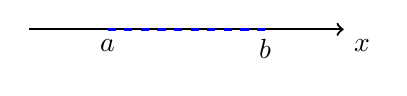
\begin{tikzpicture}
    \draw[->, thick] (-2, 0) -- (2, 0) node[anchor=north west] {$x$};

    \node[below] at (-1, 0) {$a$};
    \node[below] at (1, 0) {$b$};
    \draw[dashed, very thick, color=blue] (-1, 0) -- (1, 0);
\end{tikzpicture}
\end{center}

\subsection{Matematisk verktøy: Hyperplan og dekonstruksjonslemmaet}

For å bevise at mer komplekse elementer tilfredsstiller unisolvens, trenger vi noen matematiske verktøy. Spesielt viktig er konseptet med hyperplan og det såkalte \emph{dekonstruksjonslemmaet}.

\begin{definition}{Hyperplan}{hyperplane}
Et \textbf{hyperplan} i $\mathbb{R}^n$ er mengden av punkter $x \in \mathbb{R}^n$ som tilfredsstiller en lineær ligning:
\[
    L(x) = 0
\]
hvor $L: \mathbb{R}^n \to \mathbb{R}$ er en ikke-triviell lineær funksjon.
\end{definition}

\begin{remark}{}{}
I $\mathbb{R}^2$ er et hyperplan en linje, i $\mathbb{R}^3$ er det et plan. Vi misbruker notasjonen ved å referere til både funksjonen $L$ og mengden $\{x : L(x) = 0\}$ som \emph{hyperplanet}.
\end{remark}

\begin{lemma}{Dekonstruksjonslemmaet (DL)}{deconstruction-lemma}
La $P$ være et polynom av grad $d = \deg(P) \geq 1$ som forsvinner på hyperplanet $L$ (dvs. $P(x) = 0$ for alle $x$ slik at $L(x) = 0$). Da kan $P$ faktoriseres som:
\[
    P = L \cdot Q
\]
hvor $Q$ er et polynom av grad $\deg(Q) = d - 1$.
\end{lemma}

\begin{proof}
Uten tap av generalitet antar vi at $L(x) = x_n$ (hvor $x = (x_1, \ldots, x_{n-1}, x_n) \in \mathbb{R}^n$), det vil si at hyperplanet er beskrevet av $\{x : x_n = 0\}$.

Vi skriver $x = (\hat{x}, x_n)$ hvor $\hat{x} = (x_1, \ldots, x_{n-1})$ og $\hat{i} = (i_1, \ldots, i_{n-1})$ er en multi-indeks. Siden $\deg(P) = d$ kan vi skrive:
\[
    P(\hat{x}, x_n) = \sum_{j=0}^d \sum_{|\hat{i}| \leq d - j} C_{\hat{i}j} \hat{x}^{\hat{i}} x_n^j
\]

Siden $P$ forsvinner på hyperplanet, har vi $P(\hat{x}, 0) = 0$ for alle $\hat{x}$:
\[
    P(\hat{x}, 0) = \sum_{|\hat{i}| \leq d} C_{\hat{i}0} \hat{x}^{\hat{i}} = 0
\]

Dette impliserer at alle koeffisientene $C_{\hat{i}0} = 0$ for alle multi-indekser $\hat{i}$ med $|\hat{i}| \leq d$. Dermed kan vi omskrive $P$ som:
\[
    P(\hat{x}, x_n) = \sum_{j=1}^d \sum_{|\hat{i}| \leq d - j} C_{\hat{i}j} \hat{x}^{\hat{i}} x_n^j = x_n \underbrace{\sum_{j=1}^d \sum_{|\hat{i}| \leq d - j} C_{\hat{i}j} \hat{x}^{\hat{i}} x_n^{j-1}}_{Q(\hat{x}, x_n)}
\]

Vi har dermed $P = x_n \cdot Q = L \cdot Q$ hvor $\deg(Q) = d - 1$.
\end{proof}

\section{Triangulære elementer}

Vi ser nå på de mest brukte finite elementene i to dimensjoner: triangulære elementer. Disse bygger på trekanter som elementdomener.

\subsection{Lineære Lagrange-elementer}

Det enkleste og mest grunnleggende todimensjonale finite elementet er det lineære Lagrange-elementet.

\begin{definition}{Lineært Lagrange-element}{linear-lagrange-element}
La $\mathcal{K}$ være en trekant med hjørner $z_1, z_2, z_3$. Det \textbf{lineære Lagrange-elementet} er definert ved:
\begin{itemize}
    \item $\mathcal{P} = \mathbb{P}_1$, rommet av polynomer av grad høyst 1 i to variabler.
    \item $\mathcal{N} = \{N_1, N_2, N_3\}$ hvor $N_i(v) = v(z_i)$ for $i = 1, 2, 3$.
\end{itemize}
Merk at $\dim(\mathbb{P}_1) = 3$, så antallet nodale variabler matcher dimensjonen til funksjonsrommet.
\end{definition}

\begin{center}
 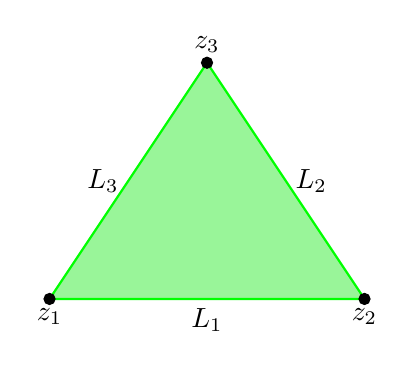
\begin{tikzpicture}
    \draw[thick, color=green, fill=green!90!black, fill opacity=0.4] (0, 0) -- (4, 0) -- (2, 3) -- cycle;
    \node[below] at (0, 0) {$z_1$};
    \node[below] at (4, 0) {$z_2$};
    \node[above] at (2, 3) {$z_3$};

    \filldraw[black] (0, 0) circle (2pt);
    \filldraw[black] (4, 0) circle (2pt);
    \filldraw[black] (2, 3) circle (2pt);

    % Include labels for edges L_i
    \node[below] at (2, 0) {$L_1$};
    \node[right] at (3, 1.5) {$L_2$};
    \node[left] at (1, 1.5) {$L_3$};
\end{tikzpicture}
\end{center}

I figuren representerer $\cdot$ nodene $z_i$ og $L_i$ representerer kantene (kanten motsatt hjørne $i$).

\begin{proof}[Bevis at $\mathcal{N}$ bestemmer $\mathbb{P}_1$ (unisolvens)]
La $L_1, L_2, L_3$ være lineære funksjoner som beskriver kantene til trekanten $\mathcal{K}$, det vil si $L_i = 0$ på kant nummer $i$.

Anta at $P \in \mathbb{P}_1$ tilfredsstiller $N_i(P) = 0$ for $i = 1, 2, 3$, det vil si $P$ forsvinner på alle tre hjørnene.

Siden $P$ er lineær i to variabler, er restriksjonen $P|_{L_1}$ et lineært polynom i én variabel langs kanten $L_1$. Dette polynomet forsvinner på to punkter (hjørnene $z_2$ og $z_3$), og det eneste lineære polynomet med to nullpunkter er nullpolynomet. Dermed har vi $P|_{L_1} \equiv 0$.

Ved dekonstruksjonslemmaet \ref{lem:deconstruction-lemma} kan vi skrive $P = L_1 \cdot c$ hvor $c$ er en konstant (siden $\deg(P) = 1$ impliserer $\deg(c) = 0$).

Men $P(z_1) = 0$ og $L_1(z_1) \neq 0$ (siden $z_1$ ikke ligger på kant $L_1$), så:
\[
    P(z_1) = c \cdot L_1(z_1) = 0 \quad \implies \quad c = 0
\]

Derfor er $P \equiv 0$, og vi konkluderer med at $\mathcal{N}$ bestemmer $\mathbb{P}_1$.
\end{proof}

\begin{remark}{}{}
Valget av hjørnepunktene som noder er ikke unikt, men det er den mest naturlige og brukte konfigurasjonen. Et annet gyldig valg kunne for eksempel vært å bruke midtpunktene på kantene som noder.
\end{remark}

\begin{center}
    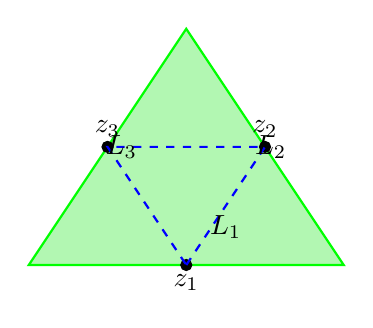
\begin{tikzpicture}
    \draw[thick, color=green, fill=green!90!black, fill opacity=0.3] (0, 0) -- (4, 0) -- (2, 3) -- cycle;
    \node[below] at (2, 0) {$z_1$};
    \node[above] at (3, 1.5) {$z_2$};
    \node[above] at (1, 1.5) {$z_3$};

    \filldraw[black] (2, 0) circle (2pt);
    \filldraw[black] (3, 1.5) circle (2pt);
    \filldraw[black] (1, 1.5) circle (2pt);

    % dashed lines between nodes
    \draw[dashed, thick, color=blue] (2, 0) -- (3, 1.5) -- (1, 1.5) -- cycle;

    % Include labels for edges L_i
    \node[below] at (2.5, 0.75) {$L_1$};
    \node[right] at (2.75, 1.5) {$L_2$};
    \node[left] at (1.5, 1.5) {$L_3$};
\end{tikzpicture}
\end{center}

\subsection{Kvadratiske Lagrange-elementer}

Vi generaliserer nå til høyere ordens polynomer.

\begin{example}{Triangulært $\mathbb{P}_2$-element}{p2-triangle-element}
La $\mathcal{K}$ være en trekant med hjørner $z_1, z_2, z_3$ og kantmidtpunkter $z_4, z_5, z_6$. Det \textbf{kvadratiske Lagrange-elementet} er definert ved:
\begin{itemize}
    \item $\mathcal{P} = \mathbb{P}_2$, rommet av polynomer av grad høyst 2 i to variabler.
    \item $\mathcal{N} = \{N_1, \ldots, N_6\}$ hvor:
    \[
        N_i(v) =
        \begin{cases}
            v(z_i), & i = 1, 2, 3 \quad \text{(hjørner)} \\
            v(z_i), & i = 4, 5, 6 \quad \text{(kantmidtpunkter)}
        \end{cases}
    \]
\end{itemize}
Merk at $\dim(\mathbb{P}_2) = 6$, så antallet noder er riktig.
\end{example}

\begin{center}
    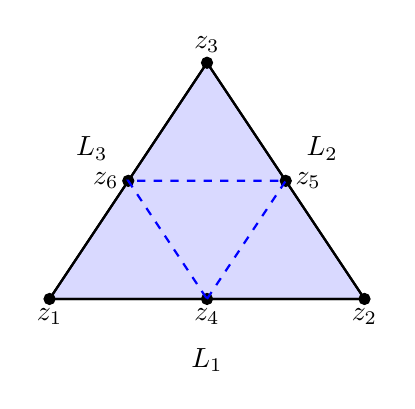
\begin{tikzpicture}
    \draw[thick, fill=blue!50, fill opacity=0.3] (0, 0) -- (4, 0) -- (2, 3) -- cycle;
    \draw[thick] (0, 0) -- (4, 0) -- (2, 3) -- cycle;
    \node[below] at (0, 0) {$z_1$};
    \node[below] at (4, 0) {$z_2$};
    \node[above] at (2, 3) {$z_3$};
    \node[below] at (2, 0) {$z_4$};
    \node[right] at (3, 1.5) {$z_5$};
    \node[left] at (1, 1.5) {$z_6$};

    \filldraw[black] (0, 0) circle (2pt);
    \filldraw[black] (4, 0) circle (2pt);
    \filldraw[black] (2, 3) circle (2pt);
    \filldraw[black] (2, 0) circle (2pt);
    \filldraw[black] (3, 1.5) circle (2pt);
    \filldraw[black] (1, 1.5) circle (2pt);

    % dashed lines between midpoints
    \draw[dashed, thick, color=blue] (2, 0) -- (3, 1.5) -- (1, 1.5) -- cycle;

    % Include labels for edges L_i
    \node[below] at (2, -0.5) {$L_1$};
    \node[above right=4pt] at (3, 1.5) {$L_2$};
    \node[above left=4pt] at (1, 1.5) {$L_3$};
\end{tikzpicture}
\end{center}

\begin{proof}[Bevis at $\mathcal{N}$ bestemmer $\mathbb{P}_2$]
La $L_1, L_2, L_3$ være lineære funksjoner som beskriver kantene til trekanten.

Anta at $P \in \mathbb{P}_2$ tilfredsstiller $N_i(P) = 0$ for alle $i = 1, \ldots, 6$.

Restriksjonen $P|_{L_1}$ er et kvadratisk polynom i én variabel som forsvinner på tre punkter: $z_2$, $z_3$ og $z_6$ (kantmidtpunktet). Et kvadratisk polynom med tre nullpunkter må være identisk null, så $P|_{L_1} \equiv 0$.

Ved dekonstruksjonslemmaet har vi:
\[
    P = L_1 \cdot Q_1
\]
hvor $\deg(Q_1) = \deg(P) - 1 = 1$.

Nå ser vi på kant $L_2$. Siden $P|_{L_2} = 0$ har vi:
\[
    L_1 Q_1|_{L_2} = 0
\]

For alle punkter på $L_2$ unntatt muligens $z_3$ (som også ligger på $L_1$), har vi $L_1 \neq 0$, så $Q_1|_{L_2} = 0$ nesten overalt. Ved kontinuitet av $Q_1$ får vi $Q_1|_{L_2} \equiv 0$.

Ved dekonstruksjonslemmaet igjen:
\[
    Q_1 = L_2 \cdot Q_2
\]
hvor $\deg(Q_2) = 0$, det vil si $Q_2 = c$ er en konstant. Dermed:
\[
    P = c \cdot L_1 \cdot L_2
\]

Men $P(z_6) = 0$ og $z_6$ ligger ikke på verken $L_1$ eller $L_2$ (det er midtpunktet på kant $L_3$), så:
\[
    P(z_6) = c \cdot L_1(z_6) \cdot L_2(z_6) = 0
\]

Siden $L_1(z_6) \neq 0$ og $L_2(z_6) \neq 0$, må $c = 0$. Derfor er $P \equiv 0$, og $\mathcal{N}$ bestemmer $\mathbb{P}_2$.
\end{proof}

\subsection{Generelle Lagrange-elementer}

Mønsteret vi har sett kan generaliseres til vilkårlige polynomgrader.


For et triangulært Lagrange-element av grad $k$ har vi:
\begin{itemize}
    \item $\mathcal{P} = \mathbb{P}_k$, med $\dim(\mathbb{P}_k) = \frac{1}{2}(k+1)(k+2)$.
    \item $\mathcal{N}_k = \{N_i\}_{i=1}^{\frac{1}{2}(k+1)(k+2)}$ består av:
    \begin{itemize}
        \item 3 hjørnepunkter
        \item $3(k-1)$ punkter fordelt på kantene ($(k-1)$ per kant)
        \item $\frac{1}{2}(k-1)(k-2)$ indre punkter
    \end{itemize}
\end{itemize}

De indre punktene må velges slik at unisolvens oppfylles.

\subsubsection{Kubisk Lagrange-element ($k=3$)}

For $k=3$ har vi $\dim(\mathbb{P}_3) = 10$ noder: 3 hjørner + 6 kantpunkter + 1 indre punkt.

\begin{center}
    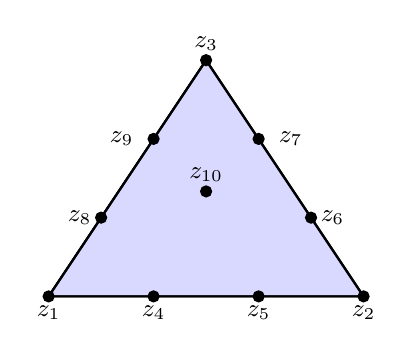
\begin{tikzpicture}[font=\small]
    \draw[thick, fill=blue!50, fill opacity=0.3] (0, 0) -- (4, 0) -- (2, 3) -- cycle;
    \draw[thick] (0, 0) -- (4, 0) -- (2, 3) -- cycle;
    \node[below] at (0, 0) {$z_1$};
    \node[below] at (4, 0) {$z_2$};
    \node[above] at (2, 3) {$z_3$};
    % Edge nodes for k=3: two per edge
    \node[below] at (1.333, 0) {$z_4$};
    \node[below] at (2.667, 0) {$z_5$};
    \node[right] at (3.333, 1) {$z_6$};
    \node[right] at (2.8, 2) {$z_7$};
    \node[left] at (0.667, 1) {$z_8$};
    \node[left] at (1.2, 2) {$z_9$};
    % Interior node
    \node[above] at (2, 1.333) {$z_{10}$};

    \filldraw[black] (0, 0) circle (2pt);
    \filldraw[black] (4, 0) circle (2pt);
    \filldraw[black] (2, 3) circle (2pt);
    \filldraw[black] (1.333, 0) circle (2pt);
    \filldraw[black] (2.667, 0) circle (2pt);
    \filldraw[black] (3.333, 1) circle (2pt);
    \filldraw[black] (2.667, 2) circle (2pt);
    \filldraw[black] (0.667, 1) circle (2pt);
    \filldraw[black] (1.333, 2) circle (2pt);
    \filldraw[black] (2, 1.333) circle (2pt);
\end{tikzpicture}

\end{center}

\begin{proof}[Bevis at $\mathcal{N}$ bestemmer $\mathbb{P}_3$ for $k=3$]
Vi viser unisolvens ved å bevise at evalueringsavbildningen
\[
    \Phi: \mathbb{P}_3 \to \mathbb{R}^{10}, \quad P \mapsto (P(z_1), P(z_2), \ldots, P(z_{10}))
\]
er injektiv, hvor $z_1, z_2, z_3$ er hjørnene, $z_4, \ldots, z_9$ er kantpunktene (to per kant), og $z_{10}$ er det indre punktet.

Siden $\dim(\mathbb{P}_3) = 10 = \dim(\mathbb{R}^{10})$, holder det å vise injektivitet for å konkludere med at $\Phi$ er en isomorfi.

\textbf{Injektivitet:} Anta at $P \in \ker(\Phi)$, det vil si $P(z_i) = 0$ for alle $i = 1, \ldots, 10$. Vi må vise at $P = 0$.

\textit{Betraktning av rommet $\mathbb{P}_3|_{\partial \mathcal{K}}$.}

La oss først betrakte $P$ på randen $\partial \mathcal{K}$. På hver kant er $P$ et enivariat polynom av grad høyst 3. La $e_j$ for $j = 1, 2, 3$ betegne de tre kantene.

På kant $e_1$ har vi $\dim(\mathbb{P}_3|_{e_1}) = 4$, og $P$ forsvinner på fire punkter på $e_1$ (nemlig de to hjørnene og to indre punkter). Siden et grad-3 polynom er entydig bestemt av fire punkter, følger det at $P|_{e_1} \equiv 0$.

Tilsvarende gir $P|_{e_2} \equiv 0$ og $P|_{e_3} \equiv 0$.

\textit{Faktorisering via rand-nullpunkter.}

La $\lambda_1, \lambda_2, \lambda_3$ være de barysentriske koordinatene for $\mathcal{K}$, som tilfredsstiller:
\[
    \lambda_1 + \lambda_2 + \lambda_3 = 1, \quad \lambda_i \geq 0 \text{ på } \mathcal{K}
\]
hvor $\lambda_i = 0$ på kant $e_i$ (kanten motsatt hjørne $i$).

Siden $P$ forsvinner på alle tre kantene, kan vi skrive:
\[
    P = \lambda_1 \lambda_2 \lambda_3 \cdot R
\]
for et polynom $R$. Vi har:
\[
    \deg(P) = 3, \quad \deg(\lambda_1 \lambda_2 \lambda_3) = 3 \quad \implies \quad \deg(R) = 0
\]

Altså er $R$ en konstant: $P = c \cdot \lambda_1 \lambda_2 \lambda_3$ for $c \in \mathbb{R}$.

\textit{Nullromsbetingelse for det indre punktet.}

Siden $z_{10}$ er et indre punkt, har vi $\lambda_i(z_{10}) > 0$ for alle $i = 1, 2, 3$. Fra $P(z_{10}) = 0$ får vi:
\[
    c \cdot \lambda_1(z_{10}) \cdot \lambda_2(z_{10}) \cdot \lambda_3(z_{10}) = 0
\]

Siden produktet av de barysentriske koordinatene er ikke-null i det indre, følger $c = 0$.

Derfor $P \equiv 0$, som viser at $\ker(\Phi) = \{0\}$, det vil si $\Phi$ er injektiv og dermed en isomorfi. Dette beviser unisolvens.
\end{proof}

\subsubsection{Kvartisk Lagrange-element ($k=4$)}

For $k=4$ har vi $\dim(\mathbb{P}_4) = 15$ noder: 3 hjørner + 9 kantpunkter + 3 indre punkter.

\begin{center}
    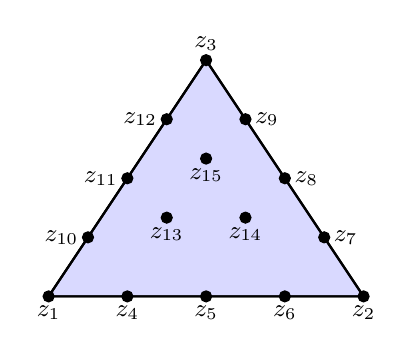
\begin{tikzpicture}[font=\small]
    \draw[thick, fill=blue!50, fill opacity=0.3] (0, 0) -- (4, 0) -- (2, 3) -- cycle;
    \draw[thick] (0, 0) -- (4, 0) -- (2, 3) -- cycle;
    \filldraw[black] (0, 0) circle (2pt) node[below] {$z_1$};
    \filldraw[black] (4, 0) circle (2pt) node[below] {$z_2$};
    \filldraw[black] (2, 3) circle (2pt) node[above] {$z_3$};
    % Edge nodes for k=4: three per edge
    \filldraw[black] (1, 0) circle (2pt) node[below] {$z_4$};
    \filldraw[black] (2, 0) circle (2pt) node[below] {$z_5$};
    \filldraw[black] (3, 0) circle (2pt) node[below] {$z_6$};
    \filldraw[black] (3.5, 0.75) circle (2pt) node[right] {$z_7$};
    \filldraw[black] (3, 1.5) circle (2pt) node[right] {$z_8$};
    \filldraw[black] (2.5, 2.25) circle (2pt) node[right] {$z_9$};
    \filldraw[black] (0.5, 0.75) circle (2pt) node[left] {$z_{10}$};
    \filldraw[black] (1, 1.5) circle (2pt) node[left] {$z_{11}$};
    \filldraw[black] (1.5, 2.25) circle (2pt) node[left] {$z_{12}$};

    % Interior nodes
    \filldraw[black] (1.5, 1) circle (2pt) node[below] {$z_{13}$};
    \filldraw[black] (2.5, 1) circle (2pt) node[below] {$z_{14}$};
    \filldraw[black] (2, 1.75) circle (2pt) node[below] {$z_{15}$};
\end{tikzpicture}

\end{center}

De tre indre punktene $z_{13}, z_{14}, z_{15}$ er valgt slik at de danner hjørnene i en mindre trekant inne i $\mathcal{K}$. Denne konfigurasjonen sikrer unisolvens.

\begin{proof}[Bevis at $\mathcal{N}$ bestemmer $\mathbb{P}_4$ for $k=4$]
Vi bruker en lineær-algebraisk tilnærming basert på dimensjonsargumenter.

\textbf{Dimensjonsanalyse.} Vi har $\dim(\mathbb{P}_4) = 15$ og definerer evalueringsavbildningen:
\[
    \Psi: \mathbb{P}_4 \to \mathbb{R}^{15}, \quad P \mapsto (P(z_1), \ldots, P(z_{15}))
\]

hvor $z_1, z_2, z_3$ er hjørnene, $z_4, \ldots, z_{12}$ er kantpunktene (tre per kant), og $z_{13}, z_{14}, z_{15}$ er indre punkter.

Det holder å vise at $\ker(\Psi) = \{0\}$ for å konkludere med at $\Psi$ er isomorfi.

\textbf{Struktur av nullrommet.} Anta $P \in \ker(\Psi)$. Vi skal vise $P = 0$ ved å bruke barysentriske koordinater.

La $\lambda_1, \lambda_2, \lambda_3: \mathcal{K} \to \mathbb{R}$ være barysentriske koordinater med:
\[
    \lambda_1 + \lambda_2 + \lambda_3 = 1, \quad \lambda_i(z_j) = \delta_{ij}, \quad \lambda_i = 0 \text{ på kant } e_i
\]

\textbf{Karakterisering av rand-polynomer.} Definer underrommet:
\[
    \mathcal{V}_{\partial} := \{P \in \mathbb{P}_4 : P|_{\partial \mathcal{K}} \equiv 0\}
\]

For hver kant $e_j$ har vi $\dim(\mathbb{P}_4|_{e_j}) = 5$, og $P$ forsvinner på 5 punkter på kant $e_j$. Med standard interpolasjonsteori følger $P|_{e_j} \equiv 0$ for alle tre kanter.

\textbf{Basis for rand-null polynomer.} Rommet $\mathcal{V}_{\partial}$ utgjøres av polynomer som kan skrives som:
\[
    \mathcal{V}_{\partial} = \text{span}\{\lambda_1 \lambda_2 \lambda_3 \cdot \lambda_i^j : i \in \{1,2,3\}, j \in \{0,1\}\}
\]

Siden $\deg(\lambda_1 \lambda_2 \lambda_3) = 3$ og vi trenger total grad $\leq 4$, kan vi kun multiplisere med lineære termer. Vi får:
\[
    \dim(\mathcal{V}_{\partial}) = 3
\]

med basis $\{\lambda_1 \lambda_2 \lambda_3 \cdot \lambda_1, \lambda_1 \lambda_2 \lambda_3 \cdot \lambda_2, \lambda_1 \lambda_2 \lambda_3 \cdot \lambda_3\}$.

\textbf{Projeksjon på internt underrom.} Siden $P \in \mathcal{V}_{\partial}$, kan vi skrive:
\[
    P = \lambda_1 \lambda_2 \lambda_3 \sum_{i=1}^3 c_i \lambda_i = \lambda_1 \lambda_2 \lambda_3 \cdot Q
\]

hvor $Q \in \mathbb{P}_1$ med $Q = c_1 \lambda_1 + c_2 \lambda_2 + c_3 \lambda_3$.

\textbf{Bestemmelse av koeffisienter via indre punkter.} For de tre indre punktene $z_{13}, z_{14}, z_{15}$ har vi:
\[
    P(z_k) = \lambda_1(z_k) \lambda_2(z_k) \lambda_3(z_k) \cdot Q(z_k) = 0, \quad k = 13, 14, 15
\]

Siden $z_k$ er indre punkter, er $\lambda_i(z_k) > 0$ for alle $i$, så:
\[
    Q(z_{13}) = Q(z_{14}) = Q(z_{15}) = 0
\]

\textbf{Injektivitet av evalueringen.} Definer restriksjonsavbildningen:
\[
    \Phi_{\text{int}}: \mathbb{P}_1 \to \mathbb{R}^3, \quad Q \mapsto (Q(z_{13}), Q(z_{14}), Q(z_{15}))
\]

Siden $z_{13}, z_{14}, z_{15}$ er ikke-kollineære (danner en egentlig trekant), og $\dim(\mathbb{P}_1) = 3$, er $\Phi_{\text{int}}$ en isomorfi. Dermed er $Q(z_{13}) = Q(z_{14}) = Q(z_{15}) = 0$ hvis og bare hvis $Q \equiv 0$.

Derfor $c_1 = c_2 = c_3 = 0$, som gir $P \equiv 0$.

\textbf{Konklusjon.} Vi har vist $\ker(\Psi) = \{0\}$, så $\Psi$ er injektiv. Siden $\dim(\mathbb{P}_4) = 15 = \dim(\mathbb{R}^{15})$, er $\Psi$ en isomorfi, og $\mathcal{N}$ bestemmer $\mathbb{P}_4$ unikt.
\end{proof}

\begin{remark}{}{}
Valget av de tre indre punktene for $k=4$ er kritisk. De må danne en ikke-degenerert trekant (være ikke-kollineære) for at beviset skal fungere. I praksis velges ofte punktene slik at de danner en likesidet trekant eller på annen måte respekterer symmetrien til det ytre elementet.
\end{remark}

\section{Hermite-elementer}

En annen viktig klasse av finite elementer er \emph{Hermite-elementer}, hvor de nodale variablene inkluderer både funksjonsverdier og deriverte.

\subsection{Kubisk Hermite-element}

\begin{example}{Kubisk Hermite-element}{cubic-hermite}
La $\mathcal{K}$ være en trekant. Det \textbf{kubiske Hermite-elementet} er definert ved:
\begin{itemize}
    \item $\mathcal{P} = \mathbb{P}_3$, med $\dim(\mathbb{P}_3) = 10$.
    \item $\mathcal{N} = \{N_1, \ldots, N_{10}\}$ hvor:
    \begin{itemize}
        \item $N_i(v) = v(z_i)$ for $i = 1, 2, 3$ (punktverdier i hjørnene)
        \item Nodale variabler for deriverte i hjørnene (typisk to retningsderiverte per hjørne)
        \item $N_{10}(v) = v(z_4)$ hvor $z_4$ er tyngdepunktet av trekanten
    \end{itemize}
\end{itemize}
\end{example}

\begin{center}
    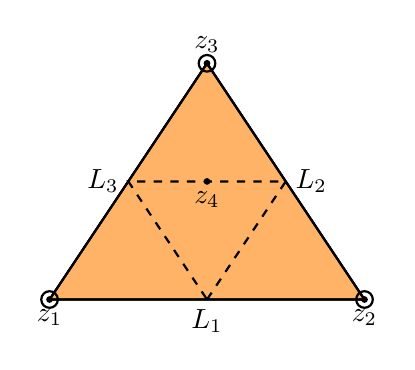
\begin{tikzpicture}
    \draw[thick, fill=orange, fill opacity=0.6] (0, 0) -- (4, 0) -- (2, 3) -- cycle;
    \draw[thick] (0, 0) -- (4, 0) -- (2, 3) -- cycle;
    \draw[thick, dashed] (2,0) -- (3, 1.5) -- (1,1.5) -- cycle;
    \draw[thick] (0, 0) circle (3pt) node[below] {$z_1$};
    \draw[thick] (4, 0) circle (3pt) node[below] {$z_2$};
    \draw[thick] (2, 3) circle (3pt) node[above] {$z_3$};
    \filldraw (2, 1.5) circle (1pt) node[below] {$z_4$};
    \filldraw (0, 0) circle (1pt);
    \filldraw (4, 0) circle (1pt);
    \filldraw (2, 3) circle (1pt);

    % Include labels for edges L_i
    \node[below] at (2, 0) {$L_1$};
    \node[right] at (3, 1.5) {$L_2$};
    \node[left] at (1, 1.5) {$L_3$};
\end{tikzpicture}

\end{center}

\begin{proof}[Bevis-skisse at $\mathcal{N}$ bestemmer $\mathbb{P}_3$]
Anta at $p \in \mathbb{P}_3$ tilfredsstiller $N_i(p) = 0$ for alle $i$.

Ved restriksjon til kant $L_1$ har vi at $p|_{L_1}$ er et kubisk polynom i én variabel som forsvinner i to punkter ($z_2$ og $z_3$), og derivertene forsvinner også i disse punktene. Dette gir fire betingelser:
\[
    \begin{cases}
        p(z_2) = 0, & p'(z_2) = 0 \\
        p(z_3) = 0, & p'(z_3) = 0
    \end{cases}
\]

hvor derivertene er tatt langs kanten. Det eneste kubiske polynomet med fire nullpunkter (teller med multiplisitet) er nullpolynomet, så $p|_{L_1} \equiv 0$.

På samme måte får vi $p|_{L_2} \equiv 0$ og $p|_{L_3} \equiv 0$.

Ved gjentatt bruk av dekonstruksjonslemmaet får vi:
\[
    p = c \cdot L_1 \cdot L_2 \cdot L_3
\]

for en konstant $c$. Men $p(z_4) = 0$ hvor $z_4$ er tyngdepunktet, og $L_i(z_4) \neq 0$ for alle $i = 1, 2, 3$. Dermed må $c = 0$, så $p \equiv 0$.
\end{proof}

\subsection{Definisjon av deriverte i nodale variabler}

For Hermite-elementer må vi spesifisere hvilke deriverte som brukes. I praksis brukes ofte \emph{retningsderiverte} langs to lineært uavhengige retninger i hvert hjørne.

\begin{center}
    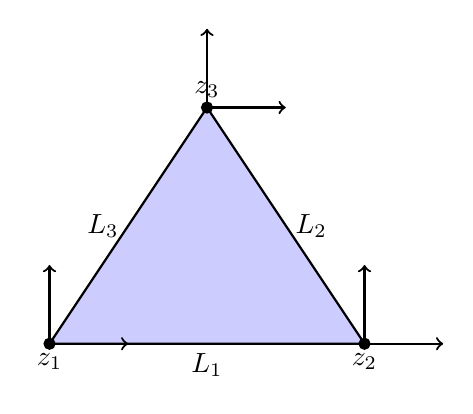
\begin{tikzpicture}
    \draw[thick, fill=blue!50, fill opacity=0.4] (0, 0) -- (4, 0) -- (2, 3) -- cycle;
    \filldraw[black] (0, 0) circle (2pt) node[below] at (0, 0) {$z_1$};
    \filldraw[black] (4, 0) circle (2pt) node[below] at (4, 0) {$z_2$};
    \filldraw[black] (2, 3) circle (2pt) node[above] at (2, 3) {$z_3$};
    \draw[->, thick, black] (0,0) -- (1,0);
    \draw[->, thick, black] (0,0) -- (0,1);
    \draw[->, thick, black] (4,0) -- (5,0);
    \draw[->, thick, black] (4,0) -- (4,1);
    \draw[->, thick, black] (2,3) -- (3,3);
    \draw[->, thick, black] (2,3) -- (2,4);

    % Include labels for edges L_i
    \node[below] at (2, 0) {$L_1$};
    \node[right] at (3, 1.5) {$L_2$};
    \node[left] at (1, 1.5) {$L_3$};
\end{tikzpicture}

\end{center}

Pilene i figuren illustrerer retningene for derivertene i hvert hjørne.

\begin{remark}{}{}
Hermite-elementer er ikke like vanlig brukt som Lagrange-elementer, men de har fordeler i enkelte anvendelser, spesielt når løsningen krever høyere glatthet.
\end{remark}

\subsection{Generelle Hermite-elementer}

For høyere grader har Hermite-elementer $\frac{1}{2}(k+1)(k+2)$ frihetsgrader, fordelt som:
\begin{itemize}
    \item 3 hjørner med punktverdier
    \item 6 deriverte (to per hjørne)
    \item $3(k-3)$ punkter på kantene
    \item $\frac{1}{2}(k-2)(k-1)$ indre punkter
\end{itemize}

\end{document}
